\documentclass{article}
\usepackage{enumerate}
\usepackage[dvipsnames]{xcolor}

% -----------------------------------------------------------------------------
% CREANDO COMANDOS
% -----------------------------------------------------------------------------
\newcommand{\uno}[2]{{#1}+{#2}}
\newcommand{\bim}[3][a][b]{{#1}^2+{#2}^2={#3}^2}

% -----------------------------------------------------------------------------


\usepackage{Sweave}
\begin{document}
\Sconcordance{concordance:ejemplo.tex:ejemplo.Rnw:%
1 13 1 1 0 40 1 1 2 13 0 1 2 7 1}


\title{ejemplo}
\author{omarpbrasta }
\date{September 2023}

\maketitle

\section{Introduction}
\subsection{HOLA2}
\subsubsection{HOLA 3}

\begin{figure}[h]
    \centering
    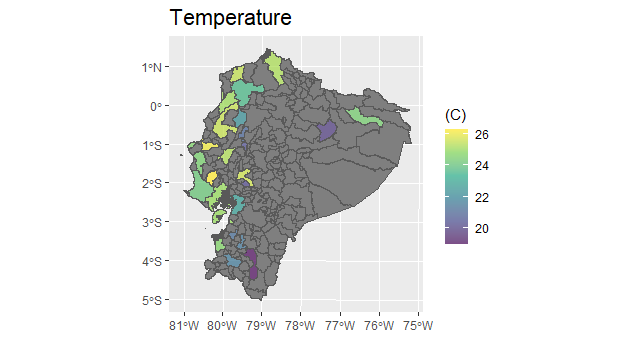
\includegraphics{Rplot.png}
    \caption{Caption}
    \label{fig:enter-label}
\end{figure}


Hola \\
como
estas

A pesar de que no existieron factores de expansión recortados, para evaluar los
diferentes niveles de recorte aplicados, se estimó los MSE de 3 indicadores: PEA,
empleo adecuado y desempleo, bajo diferentes desagregaciones como nivel
nacional, por área y por estrato de muestreo, determinando los niveles\\
“óptimos” de recorte para cada indicador investigado y para cada nivel de
desagregación analizado


\begin{tabular}{|c|c|c|}
\hline
X1 & X2 & X3 \\
\hline
1 & 2 & 3 \\
\hline
\end{tabular}

\begin{Schunk}
\begin{Sinput}
> summary(cars)
\end{Sinput}
\begin{Soutput}
     speed           dist       
 Min.   : 4.0   Min.   :  2.00  
 1st Qu.:12.0   1st Qu.: 26.00  
 Median :15.0   Median : 36.00  
 Mean   :15.4   Mean   : 42.98  
 3rd Qu.:19.0   3rd Qu.: 56.00  
 Max.   :25.0   Max.   :120.00  
\end{Soutput}
\end{Schunk}

Esto tiene color \textcolor{red}{hola que mas} \\

$\uno{w}{y}$ \\
$\bim{3}{4}{5}$\\
$\bim{1}$\\

\end{document}
